\documentclass{beamer}
%
% Choose how your presentation looks.
%
% For more themes, color themes and font themes, see:
% http://deic.uab.es/~iblanes/beamer_gallery/index_by_theme.html
%
\mode<presentation>
{
  \usetheme{default}      % or try Darmstadt, Madrid, Warsaw, ...
  \usecolortheme{crane} % or try albatross, beaver, crane, ...
  \usefonttheme{structurebold}  % or try serif, structurebold, ...
  \setbeamertemplate{navigation symbols}{}
  \setbeamertemplate{caption}[numbered]
} 

\usepackage[english]{babel}
\usepackage[utf8x]{inputenc}

\title[ML]{Machine Learning}
\author{Pawel Wocjan}
\institute{University of Central Florida}
\date{Spring 2019}

\begin{document}

\begin{frame}
  \titlepage
\end{frame}

% Uncomment these lines for an automatically generated outline.
%\begin{frame}{Outline}
%  \tableofcontents
%\end{frame}

\begin{frame}{Keras}
\begin{itemize}
\item Keras is a deep-learning framework for Python that provides a convenient way to define and train almost any kind of deep-learning model.
\item Keras has the following features:
\begin{itemize}
\item It allows the same code to run seamlessly on CPU or GPU.
\item It has a user-friendly API that makes it easy to quickly prototype deep-learning models.
\item It has built-in support for convolutional networks (for computer vision), recurrent networks (for sequence processing), and for any combination of both.
\item It supports arbitrary network architectures such as multi-input or multi-output models, and layer sharing. 
\item It is appropriate for building essentially any deep-learning model, from a generative adversarial network to a neural Turing machine.
\end{itemize}
\item Keras documentation \url{https://keras.io/}
\end{itemize}
\end{frame}

\begin{frame}{Keras, TensorFlow, Theano, and CNTK}

\begin{itemize}
\item Keras is a model-level library, providing high-level building blocks for developing deep-learning models.
\item It doesn't handle low-level operations such as tensor manipulation and differentiation. 
\item Instead, it relies on a specialized, well-optimized library to do so, serving as a backend of Keras.
\item Rather, than choosing a single tensor library and tying the implementation of Keras to that library, Keras handles the problem in a modular way:

\medskip
\begin{tabular}{|c|c|}
\hline
\multicolumn{2}{|c|}{Keras} \\ \hline
\multicolumn{2}{|c|}{TensorFlow/Theano/CNTK/ \ldots} \\ \hline
CUDA/cuDNN & Blas, Eigen \\ \hline
GPU & CPU \\ \hline
\end{tabular}
\end{itemize}
\end{frame}

\begin{frame}{Keras, TensorFlow, Theano, and CNTK}

\begin{itemize}
\item TensorFlow 

\url{https://www.tensorflow.org/}

\item Theano 
\url{http://www.deeplearning.net/software/theano/}

\item CNTK
{\small \url{https://www.microsoft.com/en-us/cognitive-toolkit/}}

\item CUDA 

\url{https://developer.nvidia.com/about-cuda}
\item cuDNN 

\url{https://developer.nvidia.com/cudnn}
\item Blas 

\url{http://www.netlib.org/blas/}
\item Eigen 

{\small \url{http://eigen.tuxfamily.org/index.php?title=Main_Page}}
\end{itemize}
\end{frame}

\begin{frame}{Developing with Keras: a quick overview}
The typical Keras workflow looks like:
\begin{itemize}
\item Define your training data: input tensors and target tensors.
\item Define a network of layers (or model) that maps your inputs to your targets.
\item Configure the learning process by choosing a loss function, an optimizer, and some metrics to monitor.
\item Iterate on your training data by calling the \texttt{fit()} function method of your model.
\end{itemize}
\end{frame}

\end{document}

%%%%%%%%%%%%%%%%%%%%%%%%%%%%%%%%%%%%%%%%%%%%%%%

\begin{frame}{Sources for Slides}

\begin{itemize}
\item I have extensively used the machine learning materials that have been prepared by Google. 

\medskip
\footnotesize{ 
\url{https://developers.google.com/machine-learning/crash-course/}
}

\item Google has licensed these materials under the Creative Commons Attribution 3.0 License.

\medskip
\footnotesize{ 
\url{https://creativecommons.org/licenses/by/3.0/}
}
\end{itemize}
\end{frame}

\begin{frame}{TensorFlow}
\begin{itemize}
    \item TensorFlow is a computational framework for building machine learning models. 
    \item TensorFlow provides a variety of different toolkits that allow you to construct models at your preferred level of abstraction. 
    \item You can use lower-level APIs to build models by defining a series of mathematical operations. 
    \item Alternatively, you can use higher-level APIs (like \texttt{tf.estimator}) to specify predefined architectures, such as linear regressors or neural networks.
    \item 
\end{itemize}
\end{frame}

\begin{frame}{TensorFlow}
\begin{itemize}
    \item The following figure shows the current hierarchy of TensorFlow toolkits:
\end{itemize}

\medskip
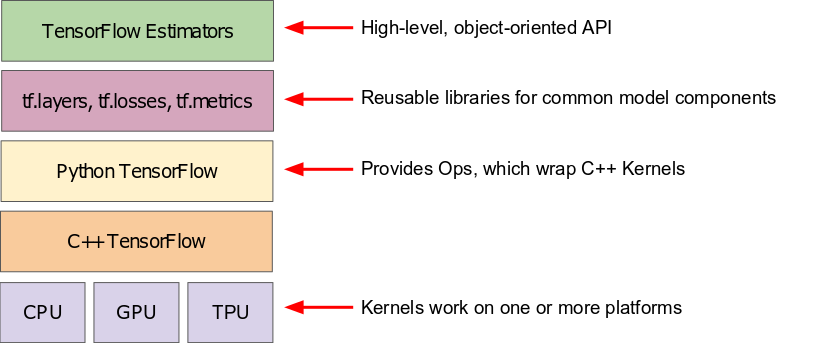
\includegraphics[width=1.0\textwidth]{images/TFHierarchy.png}
\end{frame}

\begin{frame}{TensorFlow}
\begin{itemize}
    \item The following table summarizes the purposes of the different layers:
\end{itemize}

\medskip
\begin{tabular}{|l|l|}
    \hline
    Toolkit(s) & Description \\ \hline \hline
    Estimator \texttt{tf.estimator} & High-level, OOP API \\ \hline
    \texttt{tf.layers/tf.losses/} & Libraries for common model \\
    \texttt{tf.metrics}           & components \\ \hline
    TensorFlow & Lower-level APIs \\ \hline
\end{tabular}
\end{frame}


\begin{frame}{TensorFlow}
\begin{itemize}
    \item TensorFlow consists of the following two components:
    \begin{itemize}
        \item a graph protocol buffer used to specify the  computation as a distributed graph
        \item a runtime that executes the distributed graph
    \end{itemize}
    \item These two components are analogous to
    \begin{itemize}
        \item Python code and 
        \item the Python interpreter.
    \end{itemize} 
    \item The Python interpreter is implemented on multiple hardware platforms to run Python code.
    \item Analogously, TensorFlow is implemented on multiple hardware platforms, including CPU, GPU, and TPU (Tensor Processing Unit), to run the graph.
    
    \medskip
    {\small \url{https://en.wikipedia.org/wiki/Tensor_processing_unit}}
\end{itemize}
\end{frame}

\begin{frame}{TensorFlow}
\begin{itemize}
    \item In TensorFlow, the computation is specified as a distributed graph. 
    \item Nodes in the graph represent operations. 
    \item Edges are directed and represent passing the result of an operation (a tensor) as an operand to another operation.
    \item Tensors are the primary data structure in TensorFlow programs. They are $N$-dimensional (where $N$ could be very large) data structures, most commonly scalars, vectors, or matrices. 
    \item TensorBoard is used to visualize a computational graph.
\end{itemize}
\end{frame}

\begin{frame}{TensorFlow}
\begin{itemize}
    \item Which API(s) should you use? You should use the highest level of abstraction that solves the problem. 
    \item The higher levels of abstraction are easier to use, but are also (by design) less flexible. 
    \item We recommend you start with the highest-level API first and get everything working. 
    \item If you need additional flexibility for some special modeling concerns, move one level lower. 
    \item Note that each level is built using the APIs in lower levels, so dropping down the hierarchy should be reasonably straightforward.
\end{itemize}
\end{frame}

\begin{frame}{Key Terms}
\begin{itemize}
    \item estimators
    \item graph
    \item tensor
\end{itemize}
\end{frame}

\end{document}